\subsection{Freie Schwingungen}
\begin{frame}
\frametitle{Freie Schwingungen, {\normalsize ungedämpft}}
\begin{columns}
        \begin{column}[t]{.5\linewidth}
        \begin{figure}
\begin{tikzpicture}[scale=0.6]
\fill[black!5!white] (-1,-2) rectangle (7, 3); 
\draw[->] (2.5, 2) --(4, 2);
\draw (2.5,1.8) -- (2.5, 2.2);
\draw[thin] (4,1.5)--(4,2.2);
\draw (0, 0) pic [scale=0.6] {DKbase};
\draw (0, 0) pic [scale=0.6, thick] {DKspring=4};  
\draw[thick] (4,-1.5) rectangle +(1.5, 3); 
\draw (2, -0.9) node {$k$};
\draw (4.7, 0) node {$m$};
\draw (3.25, 2.3) node {$u$};
\end{tikzpicture}


\uncover<2-5>{
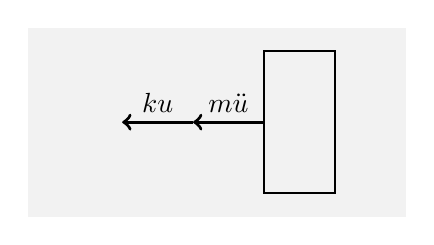
\begin{tikzpicture}[scale=0.6]
\fill[black!5!white] (-1,-2) rectangle (7, 2); 
\draw[thick] (4,-1.5) rectangle +(1.5, 3); 
\draw (3.25, 0.4) node {$m\ddot{u}$};
\draw (1.75, 0.4) node {$ku$};
\draw[<-, very thick] (2.5, 0) -- (4, 0);
\draw[<-, very thick] (1, 0) -- (2.5, 0);
\end{tikzpicture}

}
\caption*{Modell \uncover<2-5>{und Freischnitt}}
\end{figure}
        \end{column}
		\hfill
		\begin{column}[t]{.5\linewidth}
\uncover<3-5>{
		Bewegungsgleichung
\begin{equation*}
 -ku-m\ddot{u}=0
\end{equation*}
}
\uncover<4-5>{
Standardform
\begin{align*}
 \ddot{u}+\omega_0^2 u&=0\\
 \omega_0^2&=\frac{k}{m}
\end{align*}
}
\uncover<5>{
Lösung
\begin{equation*}
 u(t)=C_1\cos\omega_0 t + C_2\sin\omega_0 t
\end{equation*}
mit $C_1$, $C_2$ aus $u(t_0)=u_0$, $\dot{u}(t_0)=\dot{u}_0$
}
		\end{column}
\end{columns}
\end{frame}


\begin{frame}
\frametitle{Freie Schwingungen, {\normalsize gedämpft 1/5}}

\begin{columns}
        \begin{column}[t]{.5\linewidth}
        \begin{figure}
 \begin{tikzpicture}[scale=0.6]
 \fill[black!5!white] (-1,-3) rectangle (7, 3); 
\draw (0, 0) pic [scale=0.6] {DKbase};
\draw (0, 1) pic [scale=0.6, thick] {DKspring=4};
\draw (0,-1) pic [scale=0.6, thick] {DKdashpot=4};  
\draw[->] (2.5, 2) --(4, 2);
\draw (2.5,1.8) -- (2.5, 2.2);
\draw[thin] (4,1.5)--(4,2.2);
\draw[thick] (4,-1.5) rectangle +(1.5, 3); 
\draw (2.0, 0.1) node {$k$};
\draw (2.0,-1.9) node {$c$};
\draw (4.7, 0) node {$m$};
\draw (3.25, 2.3) node {$u$};
\end{tikzpicture}


\uncover<2-4>{
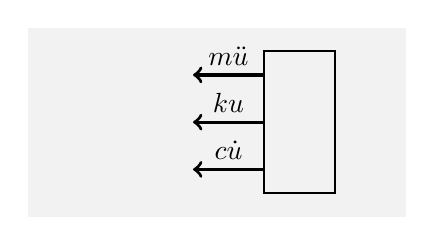
\begin{tikzpicture}[scale=0.6]
\fill[black!5!white] (-1,-2) rectangle (7, 2); 
\draw[thick] (4,-1.5) rectangle +(1.5, 3); 
\draw (3.25, 1.4) node {$m\ddot{u}$};
\draw (3.25, 0.4) node {$ku$};
\draw (3.25,-0.6) node {$c\dot{u}$};
\draw[<-, very thick] (2.5, 1) -- (4, 1);
\draw[<-, very thick] (2.5, 0) -- (4, 0);
\draw[<-, very thick] (2.5,-1) -- (4,-1);
\end{tikzpicture}

}
\caption*{Modell \uncover<2-4>{und Freischnitt}}
\end{figure}
        \end{column}
		\hfill
		\begin{column}[t]{.5\linewidth}
\uncover<3-4>{
		Bewegungsgleichung
\begin{equation*}
 -ku-c\dot{u}-m\ddot{u}=0
\end{equation*}
}
\uncover<4>{
Standardform
\begin{align*}
 \ddot{u}+2 \zeta\omega_0\dot{u}+\omega_0^2 u&=0\\
 2 \zeta\omega_0&=\frac{c}{m}\\
 \omega_0^2&=\frac{k}{m}
\end{align*}
}

		\end{column}
\end{columns}
\end{frame}


\begin{frame}
\frametitle{Freie Schwingungen, {\normalsize gedämpft 2/5}}
\begin{align*}
\ddot{u}+2 \zeta\omega_0\dot{u}+\omega_0^2 u&=0\\
u(t_0)&=u_0\\
\dot{u}(t_0)&=\dot{u}_0\\
\end{align*}
Gewöhnliche Differentialgleichung zweiter Ordnung mit konstanten Koeffizienten $\leadsto$ Exponentialansatz $u(t)=Ae^{\alpha t}$ $\leadsto$ charakteristische Gleichung
\begin{align*}
\alpha^2 + 2 \zeta\omega_0\alpha + \omega_0^2 &= 0 \\
\leadsto \alpha_{1}, \alpha_{2}&=- \zeta\omega_0\pm \omega_0\sqrt{ \zeta^2-1}
\end{align*}
\end{frame}


\begin{frame}
\frametitle{Freie Schwingungen, {\normalsize gedämpft 3/5}}
\begin{itemize}[<+->]

\item $\zeta^2>1$ überkritisch gedämpft, $\alpha_1, \alpha_2 \in \mathbb{R}$ und $\alpha_2 < \alpha_1 < 0$  
 \begin{equation*}
 u(t)=A_1 e^{\alpha_1 t}+ A_2 e^{\alpha_2 t}
 =A_1 e^{-\omega_0\left(\zeta-\sqrt{\zeta^2-1}\right)t}
 +A_2 e^{-\omega_0\left(\zeta+\sqrt{\zeta^2-1}\right)t}
 \end{equation*}
 
 \item $\zeta^2<1$ unterkritisch gedämpft, $\alpha_1, \alpha_2 \in \mathbb{C}$ und $\alpha_1=\bar{\alpha}_2$  
 \begin{equation*}
 u(t)= A_1 e^{\alpha_1 t}+ A_2 e^{\alpha_2 t}
 =e^{-\delta t}\bigl( C_1\cos\omega_1 t + C_2\sin\omega_1 t \bigr)
 \end{equation*}
 mit $\omega_1=\omega_0\sqrt{1- \zeta^2}$ und $\delta=\zeta\omega_0$, Herleitung folgt auf nächster Folie.
 
 \item $\zeta^2=1$ kritisch gedämpft,  $\alpha_1, \alpha_2 \in \mathbb{R}$ und $\alpha_1=\alpha_2<0$  
 \begin{equation*}
 u(t)= \bigl( A_1+A_2 t \bigr)e^{\alpha t}
 = \bigl( A_1+A_2 t \bigr)e^{-\zeta\omega_0 t}
 \end{equation*}
 Knobelspaß, siehe \textsl{mehrfache Nullstellen der charakteristischen Gleichung}!
\end{itemize}

\end{frame}

\begin{frame}
\frametitle{Freie Schwingungen, {\normalsize gedämpft 4/5}}
%Erinnerung Euler-Formel $e^{ix}=\cos x + i \sin x$ 
Herleitung der Lösung des unterkritisch gedämpften Falls
\begin{align*}
 u(t)  &=A_1 e^{-\omega_0\left( \zeta-\sqrt{ \zeta^2-1}\right)t}
  +A_2 e^{-\omega_0\left( \zeta+\sqrt{ \zeta^2-1}\right)t}\\
  &=A_1 e^{-\omega_0 \zeta t}e^{\omega_0 \sqrt{ \zeta^2-1}t}
  +A_2 e^{-\omega_0 \zeta t}e^{-\omega_0 \sqrt{ \zeta^2-1}t}\\
  &=A_1 e^{-\overbrace{\omega_0 \zeta}^{\delta} t}e^{i\overbrace{\omega_0 \sqrt{1-\zeta^2}}^{\omega_1}t}
  +A_2 e^{-\omega_0 \zeta t}e^{-i\omega_0 \sqrt{1-\zeta^2}t}\\
  &=A_1 e^{-\delta t}e^{i\omega_1t}+\mathrm{cc}(A_1) e^{-\delta t}e^{-i\omega_1t}\\
  &= e^{-\delta t}\Bigl( (A_{1R})+i A_{1I}) (\cos\omega_1 t + i \sin \omega_1 t  )\\
  & \qquad \quad +(A_{1R})-i A_{1I}) (\cos\omega_1 t - i \sin \omega_1 t)  \Bigr)\\
  &=e^{-\delta t}\bigl( \underbrace{2A_{1R}}_{C_1}\cos \omega_1 t 
  \underbrace{- 2A_{1R}}_{C_2}\sin \omega_1 t   \bigr)
 \end{align*}
\end{frame}


\begin{frame}
\frametitle{Freie Schwingungen, {\normalsize gedämpft 5/5}}

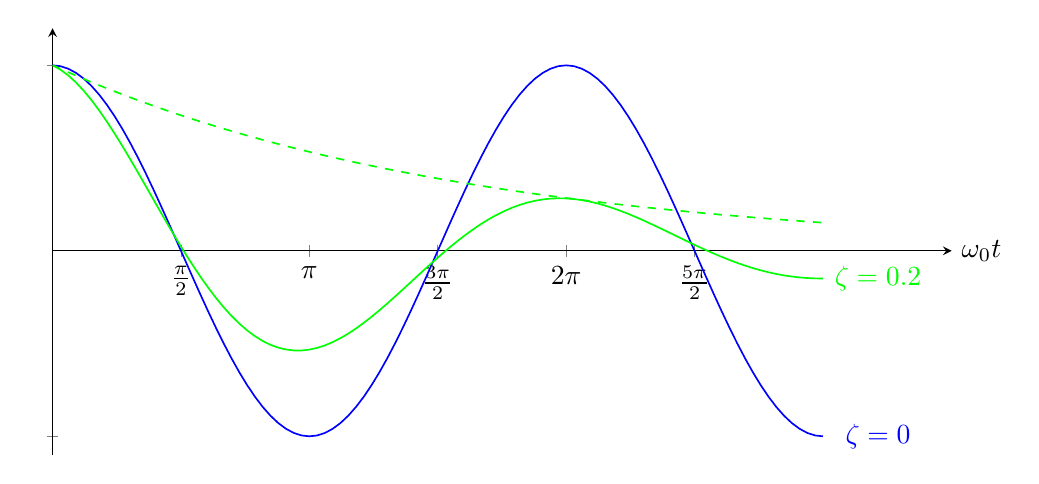
\begin{tikzpicture}
\begin{axis}[
    width=13cm, 
    height=7cm,
    axis x line=center, 
    axis y line=middle, 
    xlabel={$\omega_0 t$},
     x label style={at={(current axis.right of origin)}, right},
    samples=100,
    ymin=-1.1, ymax=1.2,
    xmin=0, xmax=11,
    domain=0:3*pi,
    xtick={ 1.5708, 3.14159, 4.7123889, 6.28318, 7.853981 },
    xticklabels={ 
    $\frac{\pi}{2}$, $\pi$, $\frac{3\pi}{2}$, $2\pi$, $\frac{5\pi}{2}$
    },
    ytick={-1,0,1},
    yticklabels={,,}
]
\addplot [mark=none, semithick, blue] {cos(deg(x))};
\addplot [mark=none, semithick, green, dashed] {exp(-0.2*x)};
\addplot [mark=none, semithick, green] {exp(-0.2*x)*cos(0.98*deg(x))};
\node[text=blue] at (axis cs:10.1,-1.0) {$\zeta=0$};
\node[text=green] at (axis cs:10.1,-0.15) {$\zeta=0.2$};
\end{axis}
\end{tikzpicture}


\end{frame}


%Einfach harmonisch

%Ungedämpfte
%Modell
%Bewergungsgleichung Lösung (fig)
% Resonanz Knobelspaß

%Gedämpfte
%FRF (fig A(f), phi(f))
%Knobelspaß 
